% ==============================================================================
% Modelo para Especificação de Projeto de Software
% Prof. Vítor E. Silva Souza - NEMO/UFES :: DI/UFES :: PPGI/UFES
%
% Baseado em abtex2-modelo-trabalho-academico.tex, v-1.9.2 laurocesar
% Copyright 2012-2014 by abnTeX2 group at http://abntex2.googlecode.com/ 
%
% This work may be distributed and/or modified under the conditions of the LaTeX 
% Project Public License, either version 1.3 of this license or (at your option) 
% any later version. The latest version of this license is in
% http://www.latex-project.org/lppl.txt.
%
% IMPORTANTE:
% Instruções encontram-se espalhadas pelo documento. Para facilitar sua leitura,
% tais instruções são precedidas por (*) -- utilize a função localizar do seu
% editor para passar por todas elas.
% ==============================================================================

% Usa o estilo abntex2, configurando detalhes de formatação e hifenização.
\documentclass[
	12pt,				
	oneside,		
	a4paper,			
	english,			% Idioma adicional para hifenização.
	french,				% Idioma adicional para hifenização.
	spanish,			% Idioma adicional para hifenização.
	brazil				% O último idioma é o principal do documento.
	]{abntex2}


%%% Importação de pacotes. %%%

% Conserta o erro "No room for a new \count". 
% O comando \reserveinserts deve ser comentado ou não, dependendo da versão do LaTeX.
\usepackage{etex}
%\reserveinserts{28}

% Usa a fonte Latin Modern.
\usepackage{lmodern}

% Seleção de códigos de fonte.
\usepackage[T1]{fontenc}

% Codificação do documento em Unicode.
\usepackage[utf8]{inputenc}

% Usado pela ficha catalográfica.
\usepackage{lastpage}

% Indenta o primeiro parágrafo de cada seção.
\usepackage{indentfirst}

% Controle das cores.
\usepackage[usenames,dvipsnames]{xcolor}

% Inclusão de gráficos.
\usepackage{graphicx}

% Melhor controle de leiaute de tabelas.
\usepackage{tabularx}
\usepackage{colortbl}
\usepackage{longtable}
\usepackage{pdflscape}

% Inclusão de páginas em PDF diretamente no documento (para uso nos apêndices).
\usepackage{pdfpages}

% Para melhorias de justificação.
\usepackage{microtype}

% Citações padrão ABNT.
\usepackage[brazilian,hyperpageref]{backref}
\usepackage[alf]{abntex2cite}	
\renewcommand{\backrefpagesname}{Citado na(s) página(s):~}		% Usado sem a opção hyperpageref de backref.
\renewcommand{\backref}{}										% Texto padrão antes do número das páginas.
\renewcommand*{\backrefalt}[4]{									% Define os textos da citação.
	\ifcase #1
		Nenhuma citação no texto.
	\or
		Citado na página #2.
	\else
		Citado #1 vezes nas páginas #2.
	\fi}

% \rm is deprecated and should not be used in a LaTeX2e document
% http://tex.stackexchange.com/questions/151897/always-textrm-never-rm-a-counterexample
\renewcommand{\rm}{\textrm}

% Inclusão de símbolos não padrão.
\usepackage{amssymb}
\usepackage{eurosym}

% Para utilizar \eqref para referenciar equações.
\usepackage{amsmath}

% Permite mostrar figuras muito largas em modo paisagem com \begin{sidewaysfigure} ao invés de \begin{figure}.
\usepackage{rotating}

% Permite customizar listas enumeradas/com marcadores.
\usepackage{enumitem}

% Permite inserir hiperlinks com \url{}.
\usepackage{bigfoot}
\usepackage{hyperref}

% Permite usar o comando \hl{} para evidenciar texto com fundo amarelo. Útil para chamar atenção a itens a fazer.
\usepackage{soulutf8}

% Colorinlistoftodos package: to insert colored comments so authors can collaborate on the content.
% (*) Indicar o nome do aluno e substituir o nome do professor se for o caso.
\usepackage[colorinlistoftodos, textwidth=20mm, textsize=footnotesize]{todonotes}
\newcommand{\aluno}[1]{\todo[author=\textbf{Aluno},color=green!30,caption={},inline]{#1}}
\newcommand{\vitor}[1]{\todo[author=\textbf{Vítor},color=red!30,caption={},inline]{#1}}

% Permite inserir espaço em branco condicional (incluído no texto final só se necessário) em macros.
\usepackage{xspace}

% Permite incluir listagens de código com o comando \lstinputlisting{}.
\usepackage{listings}
\usepackage{caption}
\DeclareCaptionFont{white}{\color{white}}
\DeclareCaptionFormat{listing}{\colorbox{gray}{\parbox{\textwidth}{#1#2#3}}}
\captionsetup[lstlisting]{format=listing,labelfont=white,textfont=white}
\renewcommand{\lstlistingname}{Listagem}
\definecolor{mygray}{rgb}{0.5,0.5,0.5}
\lstset{
	basicstyle=\scriptsize,
	breaklines=true,
	numbers=left,
	numbersep=5pt,
	numberstyle=\tiny\color{mygray}, 
	rulecolor=\color{black},
	showstringspaces=false,
	tabsize=2,
    inputencoding=utf8,
    extendedchars=true,
    literate=%
    {é}{{\'{e}}}1
    {è}{{\`{e}}}1
    {ê}{{\^{e}}}1
    {ë}{{\¨{e}}}1
    {É}{{\'{E}}}1
    {Ê}{{\^{E}}}1
    {û}{{\^{u}}}1
    {ù}{{\`{u}}}1
    {â}{{\^{a}}}1
    {à}{{\`{a}}}1
    {á}{{\'{a}}}1
    {ã}{{\~{a}}}1
    {Á}{{\'{A}}}1
    {Â}{{\^{A}}}1
    {Ã}{{\~{A}}}1
    {ç}{{\c{c}}}1
    {Ç}{{\c{C}}}1
    {õ}{{\~{o}}}1
    {ó}{{\'{o}}}1
    {ô}{{\^{o}}}1
    {Õ}{{\~{O}}}1
    {Ó}{{\'{O}}}1
    {Ô}{{\^{O}}}1
    {î}{{\^{i}}}1
    {Î}{{\^{I}}}1
    {í}{{\'{i}}}1
    {Í}{{\~{Í}}}1
}




%%% Definição de variáveis. %%%
% (*) Substituir os textos abaixo com as informações apropriadas.
\titulo{Eventu}
\autor{Thaliys Antunes Daré, Gabriel Ferrari Wagnitz}
\local{Vitória, ES}
\data{\the\year}
\instituicao{
	Universidade Federal do Espírito Santo -- UFES
	\par
	Centro Tecnológico
	\par
	Departamento de Informática}
\newcommand{\subtitulo}{Documento de Projeto de Sistema}
\newcommand{\versao}{1.0}

% Define a capa.
\renewcommand{\imprimircapa}{%
	\begin{capa}%
		\center
		
		{\ABNTEXchapterfont\large\subtitulo{}}
		\vfill
		\begin{center}
			\ABNTEXchapterfont\bfseries\LARGE\imprimirtitulo
		\end{center}
		
		\vfill
		\large\imprimirlocal
		\linebreak
		\large\imprimirdata
		\vspace*{1cm}
	\end{capa}
}

% Macros específicas do trabalho.
% (*) Inclua aqui termos que são utilizados muitas vezes e que demandam formatação especial.
% Exemplo: Java com TM (trademark) em superscript.
% Use sempre \xspace para que o LaTeX inclua espaço em branco após a macro somente quando necessário.
\newcommand{\java}{Java\texttrademark\xspace}




%%% Configurações finais de aparência. %%%

% Altera o aspecto de algumas cores.
\definecolor{blue}{RGB}{41,5,195}
\definecolor{lightgray}{gray}{0.9}

% Informações do PDF.
\makeatletter
\hypersetup{
	pdftitle={\@title}, 
	pdfauthor={\@author},
	pdfsubject={\imprimirpreambulo},
	pdfcreator={LaTeX with abnTeX2},
	pdfkeywords={abnt}{latex}{abntex}{abntex2}{trabalho acadêmico}, 
	colorlinks=true,				% Colore os links (ao invés de usar caixas).
	linkcolor=blue,					% Cor dos links.
	citecolor=blue,					% Cor dos links na bibliografia.
	filecolor=magenta,				% Cor dos links de arquivo.
	urlcolor=blue,					% Cor das URLs.
	bookmarksdepth=4
}
\makeatother

% Espaçamentos entre linhas e parágrafos.
\setlength{\parindent}{1.3cm}
\setlength{\parskip}{0.2cm}



%%% Páginas iniciais do documento: capa, folha de rosto, ficha, resumo, tabelas, etc. %%%

% Compila o índice.
\makeindex

% Inicia o documento.
\begin{document}

% Retira espaço extra obsoleto entre as frases.
\frenchspacing

% Inclui o brasão da UFES.
\begin{figure}[h]
  \centering
  
\includegraphics[scale=0.055]{brasao.jpg}
  \label{ppts3}
\end{figure} 

% Capa do trabalho.
\imprimircapa


% (*) Incluir linhas no registro de alterações a cada nova versão.
\begin{center}
	{\large\bfseries Registro de Alterações:}
	
	\vspace{0.5cm}
	\begin{tabular}{|c|p{45mm}|c|p{60mm}|} \hline
		
		\textbf{Versão} & \textbf{Responsável} & \textbf{Data}  & \textbf{Alterações} \\ \hline   
		
		1.0  & Gabriel Ferrari Wagnitz e Thaliys Daré & 21/04/2024 & Versão inicial. \\\hline 
            2.0  & Gabriel Ferrari Wagnitz e Thaliys Daré & 08/06/2024 & Revisado. \\\hline 
	\end{tabular}
\end{center}
\newpage



%%% Início da parte de conteúdo do documento. %%%
% Marca o início dos elementos textuais.
\textual

% Inclusão dos capítulos como seções (sem quebra de página).
\begingroup
\let\clearpage\relax

% ==============================================================================
% Projeto de Sistema - Nome do Aluno
% Capítulo 1 - Introdução
% ==============================================================================
\chapter{Introdução}
\label{sec-intro}
\vspace{-1cm}

Este documento apresenta o projeto (\textit{design}) do sistema \emph{\imprimirtitulo}. 
O projeto consiste no desenvolvimento de uma aplicação web para organizadores de eventos acadêmicos. Eventos acadêmicos possuem necessidades particulares que não são normalmente supridas por sistemas de vendas de ingressos, que geralmente tem foco em eventos culturais e shows. Por isso, entendemos como necessário desenvolver uma plataforma voltada especificamente para o público universitário.

Os principais diferenciais do sistema Eventu são o suporte à multiplas atividades paralelas, em que os participantes dispõem de diversas atividades para escolher e o sistema faz a gestão da grade de programação, e a API para controle de presença, em que a participação numa programação pode ser registrada com auxilio da integração à um sistema de catracas.

Este documento está organizado da seguinte forma: 
a Seção~\ref{sec-plataforma} apresenta a plataforma de software utilizada na implementação do sistema;
a Seção~\ref{sec-arquitetura} apresenta a arquitetura de software; por fim, 
a Seção~\ref{sec-frameweb} apresenta os modelos FrameWeb que descrevem os componentes da arquitetura.

O projeto foi desenvolvido por Thaliys Antunes Daré e Gabriel Ferrari Wagnitz.


\vspace*{1.5cm}

% ==============================================================================
% Projeto de Sistema - Nome do Aluno
% Capítulo 2 - Plataforma de Desenvolvimento
% ==============================================================================
\chapter{Plataforma de Desenvolvimento}
\label{sec-plataforma}
\vspace{-1cm}
Para o projeto serão utilizadas as tecnologias e bibliotecas recomendadas pelo Spring Framework em seu projeto \textit{Spring Initializr}\footnote{https://start.spring.io/}. O \textit{Spring Initializr} é uma ferramenta do Spring para facilitar a configuração inicial do projeto, facilitando a inclusão de bibliotecas para diversos propósitos.


%=======================================================================================================
%			Tabela de Plataforma de Desenvolvimento e Tecnologias Utilizadas
%=======================================================================================================

Na Tabela~\ref{tabela-plataforma} são listadas as tecnologias utilizadas no desenvolvimento da ferramenta, bem como o propósito de sua utilização.

\begin{footnotesize}
\begin{longtable}{|p{1.8cm}|c|p{5cm}|p{6.3cm}|}
	\caption{Plataforma de Desenvolvimento e Tecnologias Utilizadas.}	
	\label{tabela-plataforma}\\\hline

	\rowcolor{lightgray}
	\textbf{Tecnologia} & \textbf{Versão} & \textbf{Descrição} & \textbf{Propósito} \\\hline 
	\endfirsthead
	\hline
	\rowcolor{lightgray}
	\textbf{Tecnologia} & \textbf{Versão} & \textbf{Descrição} & \textbf{Propósito} \\\hline 
	\endhead
		
	Spring Framework & 3.2.4 & Framework de inversão de controle e injeção de dependência. Possui um conjunto de APIs para auxiliar em diversas etapas do desenvolvimento de grandes sistemas web & Redução da complexidade do desenvolvimento, implantação e gerenciamento de aplicações Web a partir de seus componentes de infra-estrutura prontos para o uso. \\ \hline

	Java & 21 & Linguagem de programação orientada a objetos e independente de plataforma. & Escrita do código-fonte das classes que compõem o sistema. \\\hline
	
	Spring Data JPA & 3.2.4 & API para persistência de dados por meio de mapeamento objeto/relacional. & Persistência dos objetos de domínio sem necessidade de escrita dos comandos SQL. \\\hline
  
	Thymeleaf & 3.1.2 &  Ferramenta para criação de (\textit{templates}) XML/XHTML/HTML5 integrada ao Spring & Reutilização da estrutura visual comum às paginas, facilitando a manutenção do padrão visual do sistema. \\\hline

    TailwindCSS & 3.4.3 & Framework de classes CSS processadas em tempo de compilação & Facilitar a estilização de páginas web responsivas \\\hline
		
	MySQL Server & 8.3 & Sistema Gerenciador de Banco de Dados Relacional gratuito. & Armazenamento dos dados manipulados pela ferramenta. \\\hline
	
	Tomcat & 10.1.19 & Servidor de Aplicações Imbutido no Spring Boot. & Fornecimento de implementação das APIs citadas acima e hospedagem da aplicação Web, dando acesso aos usuários via HTTP. \\\hline
\end{longtable}
\end{footnotesize}






%=======================================================================================================
%			Tabela de Softwares de Apoio ao Desenvolvimento do Projeto
%=======================================================================================================

Na Tabela~\ref{tabela-software} vemos os softwares que apoiaram o desenvolvimento de documentos e também do código fonte.

\begin{footnotesize}
\begin{longtable}{|p{2.5cm}|c|p{5cm}|p{5.5cm}|}
	\caption{Softwares de Apoio ao Desenvolvimento do Projeto}	
	\label{tabela-software}\\\hline
	
	\rowcolor{lightgray}
	\textbf{Tecnologia} & \textbf{Versão} & \textbf{Descrição} & \textbf{Propósito} \\\hline 
	\endfirsthead
	\hline
	\rowcolor{lightgray}
	\textbf{Tecnologia} & \textbf{Versão} & \textbf{Descrição} & \textbf{Propósito} \\\hline 
	\endhead
	 
	FrameWeb Plugin & 1.0 & Plugin do VisualParadigm para o método FrameWeb. & Criação dos modelos de Entidades, Aplicação, Persistência e Navegação. \\\hline

    VisualParadigm & 17.1 & Ferramenta de modelagem UML & Criação de Diagramas de Classe  \\\hline

	Overleaf  & - & Editor Online do \LaTeX & Documentação do projeto arquitetural do sistema. \\\hline           
	
	Apache Maven & 3.6 & Ferramenta de gerência/construção de projetos de software. & Obtenção e integração das dependências do projeto. \\\hline
	
	Spring Initializr & - & Ferramenta de geração inicial de projeto Spring. & Automação de configuração \\\hline
 
\end{longtable}
\end{footnotesize}

\vspace*{1.5cm}


\chapter{Arquitetura de Software}
\label{sec-arquitetura}
\vspace{-1cm}

A Figura~\ref{figura-arquitetura} mostra a arquitetura do sistema \emph{\imprimirtitulo}.

\begin{figure}[h]
	\centering
	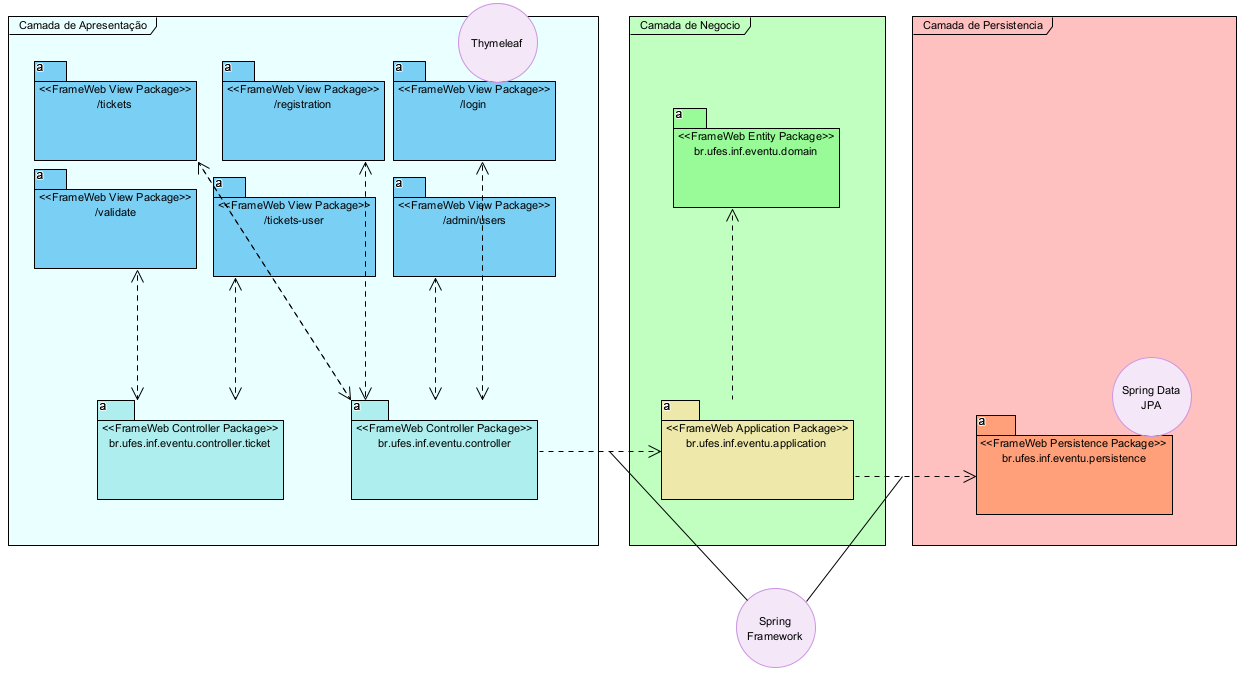
\includegraphics[width=0.8\textwidth]{figuras/Arquitetura.PNG}
	\caption{Arquitetura de Software.}
	\label{figura-arquitetura}
\end{figure}

O sistema \emph{\imprimirtitulo} adota a arquitetura Model-View-Controller (MVC)\cite{fowler:book02} para prover organização, modularidade e separação de conceitos (do inglês \textit{separation of concerns}, SoC). Além disso, a escolha da arquitetura MVC torna-se prática, dado o grande suporte que o framework Spring provê à esta arquitetura.

O sistema \emph{\imprimirtitulo} implementa cada um dos módulos MVC da seguinte forma:

\textbf{Modelo}: No núcleo do sistema, o Modelo encapsula os dados e regras de negócio, gerenciando o acesso e a manipulação de informações sobre eventos, palestrantes, participantes e inscrições. Nele estão os pacotes do modelo de aplicação (ex: ManageAttractionServiceImpl, AuthenticateUserServiceImpl), classes de dominio (ex: Ticket, User, Attraction) e de persistencia (ex: TicketJPADAO, UserJPADAO)

\textbf{Visão}: Representado pelas visualizações geradas por templates Thymeleaf e Tailwind CSS, a camada de Visão apresenta os dados do Modelo para os usuários, permitindo visualização, interação e manipulação de informações.

\textbf{Controlador}: O Controlador atua como intermediário, recebendo requisições do usuário, fazendo validação dos dados de entrada e direcionando-as para o Modelo e recuperando os dados processados para apresentá-los na Visão. As classes TicketController e UserController fazem parte da camada Controlador.
\vspace*{1.5cm}


\chapter{Modelagem FrameWeb}
\label{sec-frameweb}
\vspace{-1cm}

\emph{\imprimirtitulo} é um sistema Web cuja arquitetura utiliza \textit{frameworks} comuns no desenvolvimento para esta plataforma. Desta forma, o sistema pode ser modelado utilizando a abordagem FrameWeb~\cite{souza-celebratingfalbo20}.

A Tabela~\ref{tabela-frameworks} indica os \textit{frameworks} presentes na arquitetura do sistema que se encaixam em cada uma das categorias de \textit{frameworks} que FrameWeb dá suporte. Em seguida, os modelos FrameWeb são apresentados para cada camada da arquitetura.


\begin{footnotesize}
	\begin{longtable}{|c|c|}
		\caption{\textit{Frameworks} da arquitetura do sistema separados por categoria.}
		\label{tabela-frameworks}\\\hline
		
		\rowcolor{lightgray}
		\textbf{Categoria de \textit{Framework}} & \textbf{\textit{Framework} Utilizado} \\\hline 
		\endfirsthead
		\hline
		\rowcolor{lightgray}
		\textbf{Categoria de \textit{Framework}} & \textbf{\textit{Framework} Utilizado} \\\hline 
		\endhead

		Controlador Frontal & Spring Framework \\\hline

		Injeção de Dependências & Spring Framework \\\hline

		Mapeamento Objeto/Relacional & Spring Data JPA \\\hline

		Segurança & Spring Security \\\hline
	\end{longtable}
\end{footnotesize}




\section{Camada de Negócio}
\label{sec-frameweb-negocio}

\begin{figure}[h]
	\centering
	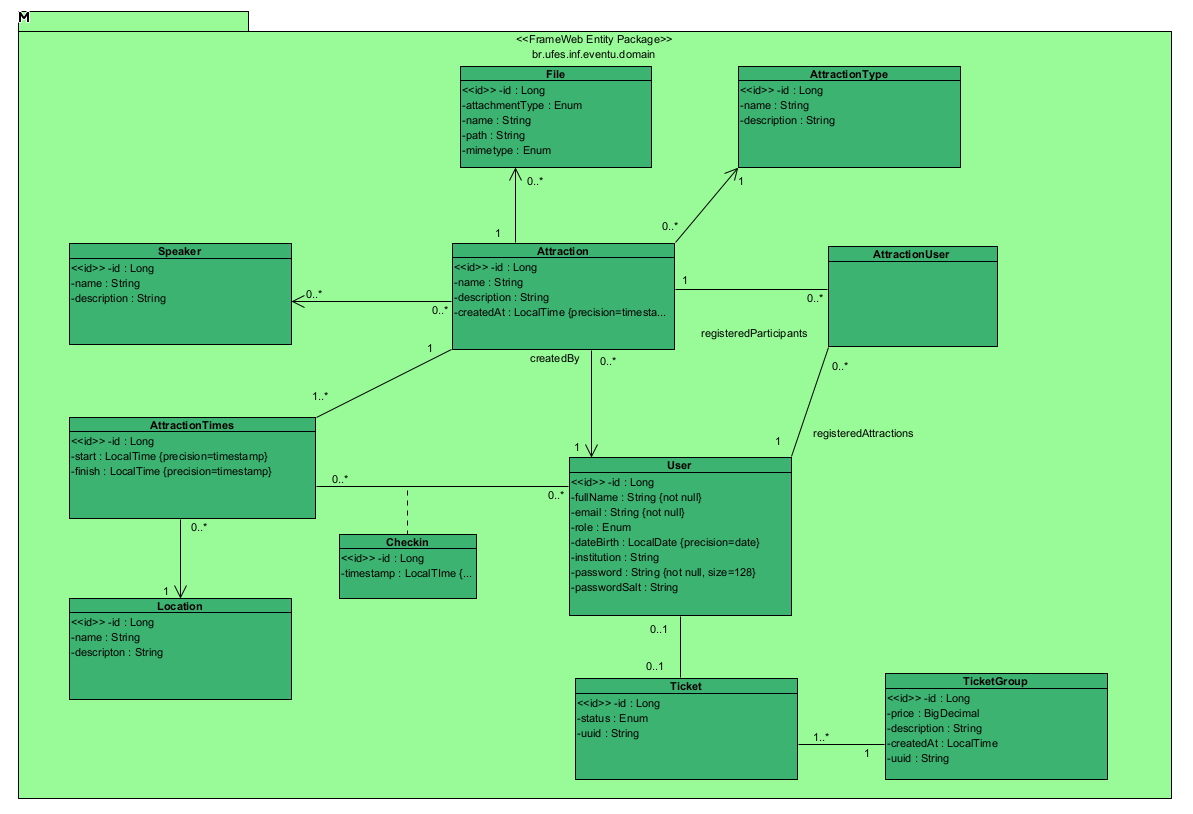
\includegraphics[width=0.8\textwidth]{figuras/ClassesDeDominio.PNG}
	\caption{Modelo de Entidades.}
	\label{figura-dominio}
\end{figure}

\textbf{Attraction}: Representa uma atração em um evento, como palestra, workshop ou visita técnica.

\textbf{Speaker}: Representa um palestrante ou outro profissional que participará de uma atração.

\textbf{File}: Representa um arquivo armazenado no sistema, como material de apresentação ou foto.

\textbf{AttractionType}: Representa o tipo de atração, como palestra, workshop ou visita técnica.

\textbf{User}: Representa um usuário do sistema, como participante, organizador ou staff.

\textbf{Ticket}: Representa um ingresso para um evento, com informações como tipo de ingresso, valor e local.

\textbf{TicketGroup}: Representa um grupo de ingressos, permitindo a emissão de vários ingressos de uma vez com um identificador comum.

\textbf{CheckIn}: Classe de relacionamento entre o horario da atração e um usuário, utilizada para registro de presença.

\textbf{CheckIn}: Classe de relacionamento entre o horario da atração e um usuário, utilizada para registro de presença.



\section{Camada de Acesso a Dados}
\label{sec-frameweb-dados}


\begin{figure}[h]
	\centering
	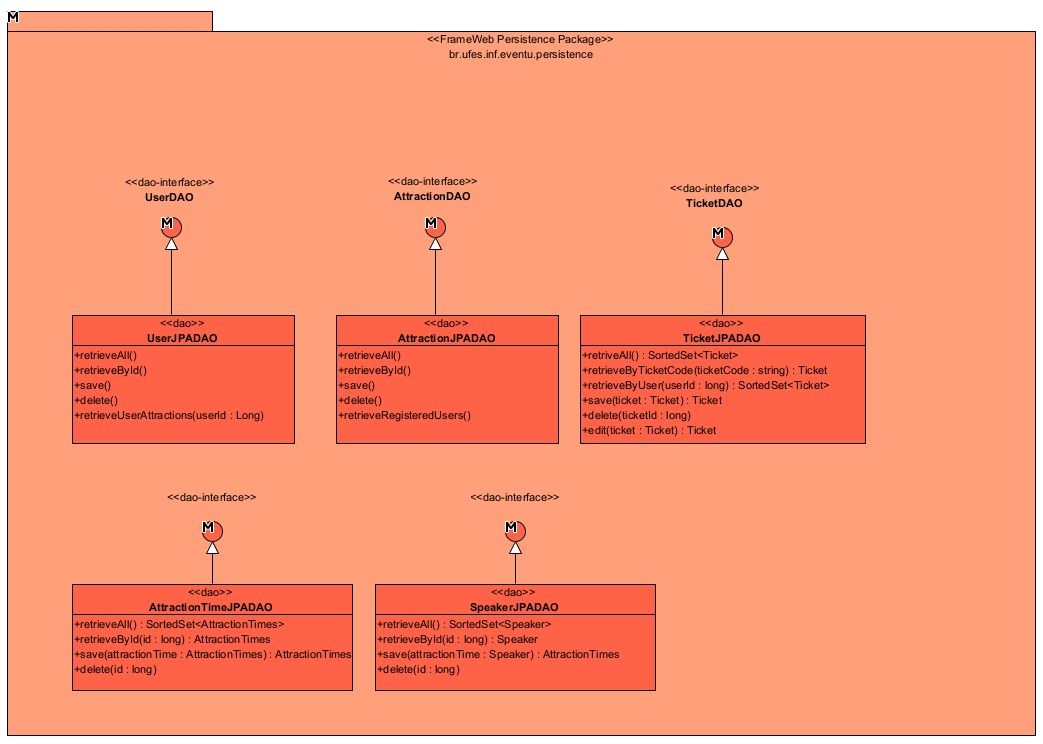
\includegraphics[width=0.8\textwidth]{figuras/ClassesDePersistencia.PNG}
	\caption{Modelo de Persistencia.}
	\label{figura-persistencia}
\end{figure}

Além da implementação de funcionalidades CRUD (do inglês: Criação, Consulta, Atualização e Destruição), podemos ressaltar na camada de acesso a dados algumas outras operações:

\textbf{TicketJPADAO}: +retireveByTicketCode - Operação responsável por encontrar o ticket no banco de dados durante o processo de validação do ingresso.

\textbf{AttractionJPADAO}: +retireveRegisteredUsers() - Operação responsável por retornar a lista de usuários inscritos em uma dada atração.


\section{Camada de Apresentação}
\label{sec-frameweb-apresentacao}

\begin{figure}[h]
	\centering
	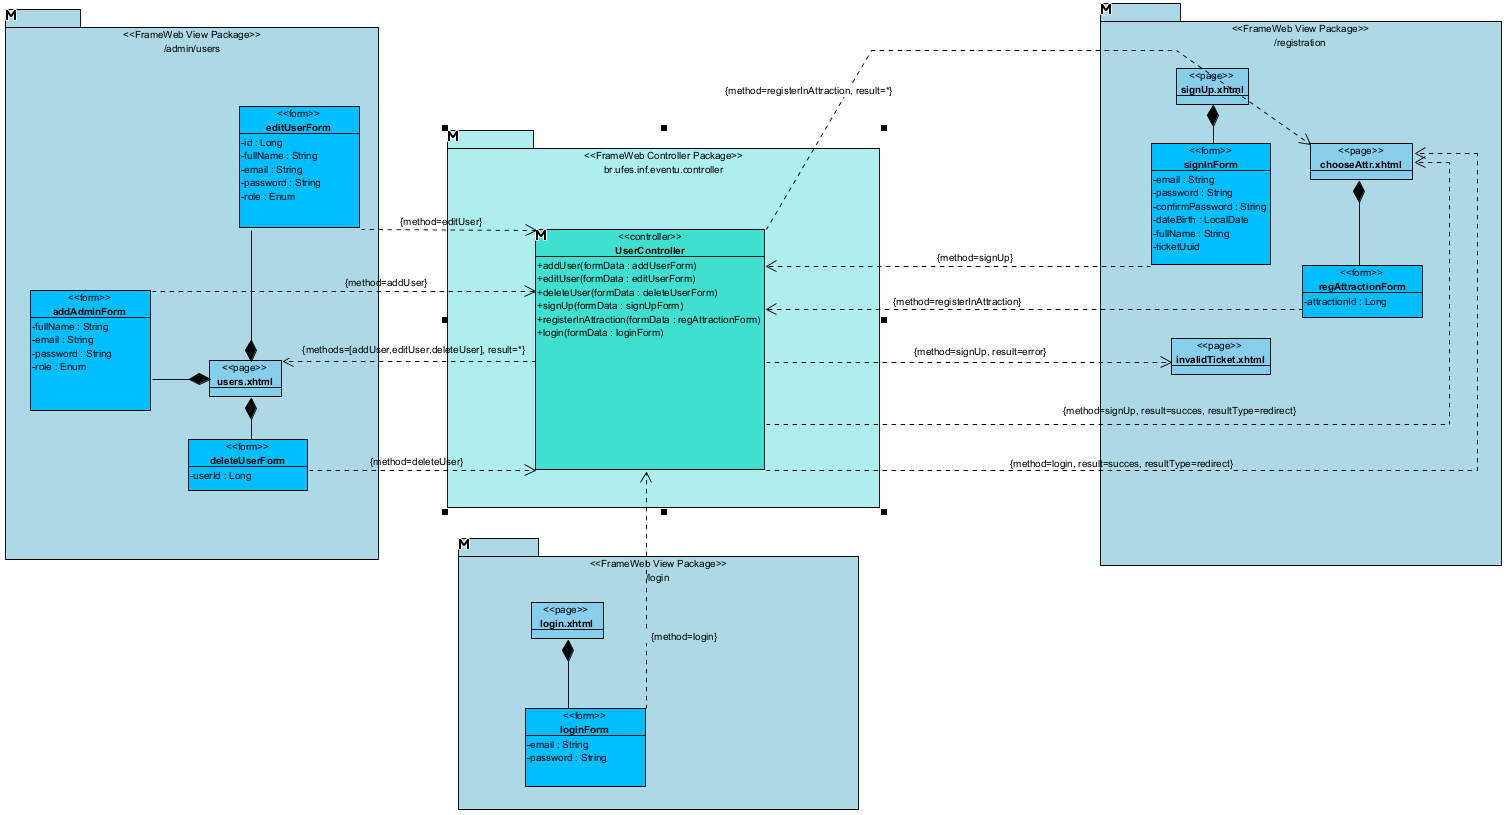
\includegraphics[width=0.8\textwidth]{figuras/ModeloNavegacaoUser.PNG}
	\caption{Modelo de Navegação - Cadastro de Usuários.}
	\label{figura-cadastrouser}
\end{figure}

A camada de apresentação é responsável pelas diversas telas do sistema. na Figura \ref{figura-cadastrouser} vemos o 3 fluxos de navegação envolvendo usuários.

Em \textbf{/admin/users} vemos o processo de gestão dos usuários por administradores.

Em \textbf{/registration} vemos o cadastro de usuários, criação de login e senha, além da validação do ticket que é comprado fora do sistema. O sistema apenas faz validação do código e a associação ao usuário. Após isso, o usuário e apresentado à tela \textbf{chooseAttr.xhtml} em que ele escolhe progressivamente  as atrações que vai participar.

Em \textbf{/registration} vemos o cadastro de usuários, criação de login e senha, além da validação do ticket que é comprado fora do sistema. O sistema apenas faz validação do código e a associação ao usuário. Após isso, o usuário e apresentado à tela \textbf{chooseAttr.xhtml} em que ele escolhe progressivamente  as atrações que vai participar.

Em \textbf{/login} vemos o fluxo de autenticação do usuário.

\begin{figure}[h]
	\centering
	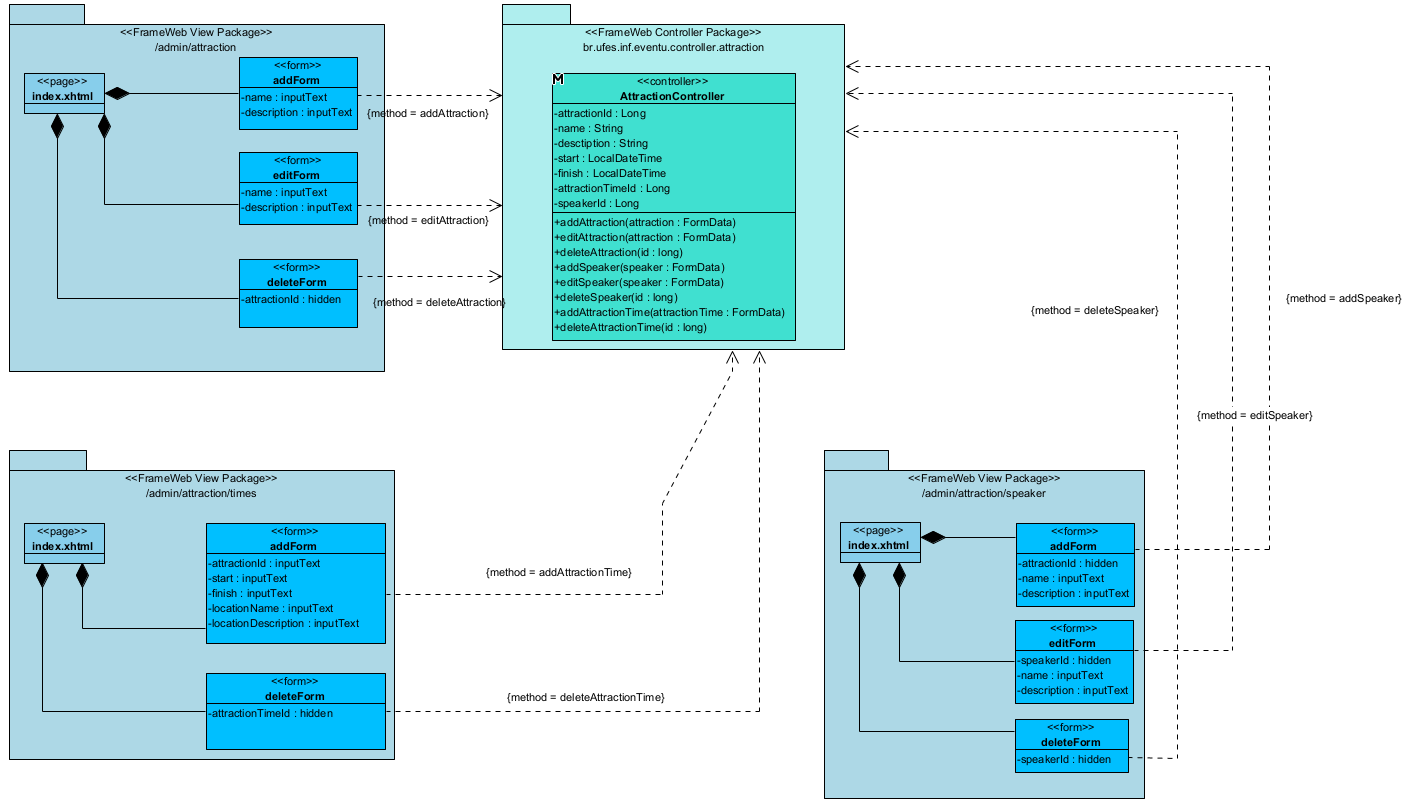
\includegraphics[width=0.8\textwidth]{figuras/ModeloNavegacaoAttr.PNG}
	\caption{Modelo de Navegação - Cadastro de Atrações.}
	\label{figura-cadastroattr}
\end{figure}


Na Figura \ref{figura-cadastroattr} vemos mais 3 fluxos de navegação, agora envolvendo envolvendo o cadastro de atrações.

O processo se assemelha a um simples CRUD, assim como na gestão de usuários por administradores. O ponto a ressaltar é que as atrações estão relacionadas à entidade palestrante e as instâncias de horário. Instancias de horário foram modeladas dessa forma para acomodar atrações que se estendam por mais de um dia, em locais diferentes. Para isso temos a classe \textit{AttractionTimes}
 
\begin{figure}[h]
	\centering
	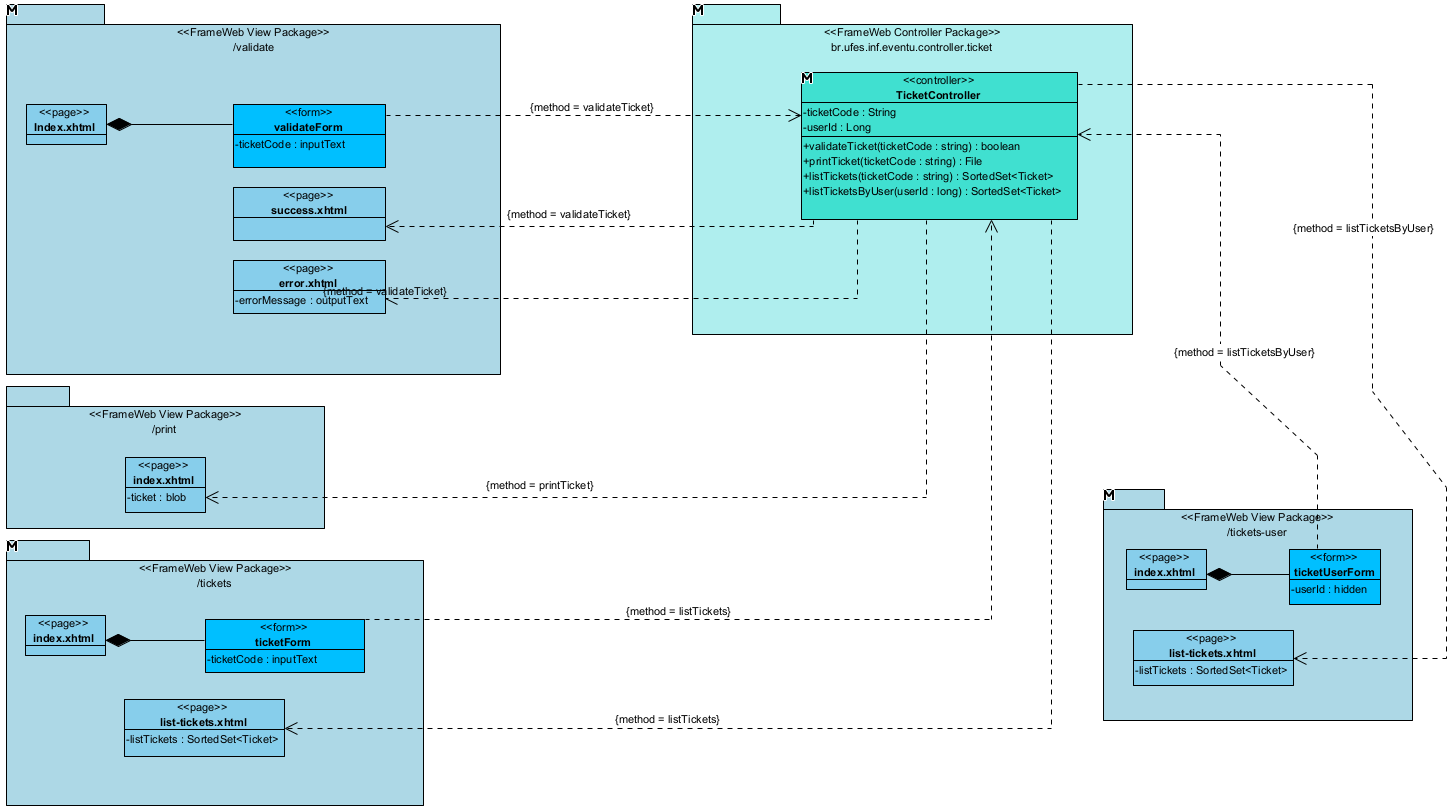
\includegraphics[width=0.8\textwidth]{figuras/ModeloNavegacaoTicket.PNG}
	\caption{Modelo de Navegação - Cadastro de Tickets.}
	\label{figura-cadastrotickets}
\end{figure}

Na Figura \ref{figura-cadastrotickets} vemos mais 4 fluxos de navegação, desta vez envolvendo envolvendo os ingressos (\textit{Tickets}).

O ponto interessante de se ressaltar é a operação \textbf{+printTicket()} que permite um administrador imprimir um ingresso, facilitando a emissão para venda física.
\endgroup



%%% Páginas finais do documento: bibliografia e anexos. %%%
% Finaliza a parte no bookmark do PDF para que se inicie o bookmark na raiz e adiciona espaço de parte no sumário.
\phantompart

% Marca o início dos elementos pós-textuais.
\postextual

% Referências bibliográficas
\bibliography{bibliografia}

% Índice remissivo.
\phantompart
\printindex

% Fim do documento.
\end{document}
